\section{Experiments}

For the experiments where swapping is needed we limited the RAM of the process to 1 mb. A limitation we achieved by using cgroups in linux - on a standard mechanical hard-drive. This was done to significantly reduce the running time of our experiments and the amount of data required. 
During the first part of our testing we did in no way manage to get the expected results. In fact they were more or less opposite of the what the theory predicted. For example running the external merge sort with one small and one large N showed the larger N to be faster! We have not managed to find an adequate explanation for this so far and it would require require more investigation to find the reason.
We have however found a solution to the above problem, which gives results that fit the theory a lot better. By including an optimization flag for our compiler (in our case we used clang) not only did the running time decrease by roughly 1/3 but the results of the test cases also align better with the expected result. 

\subsection{Stream implementations}
The tests for our streams include testing different values of the buffersize $b$, the amount of streams $k$, and with $n = 100.000.000$ (for SingleItemStreams $n$ is only 100.000 - it is simply too slow to consider a valid candidate, and therefore is discarded in the comparison). 
Each test has been run 100 times where the average is the values used in the graphs. 

\subsubsection{SingleItemStream and FStream}
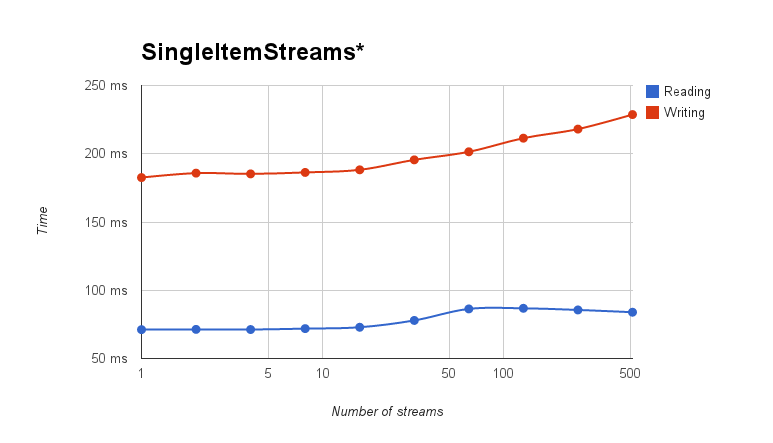
\includegraphics[width=90mm]{graphics/SIS.png}
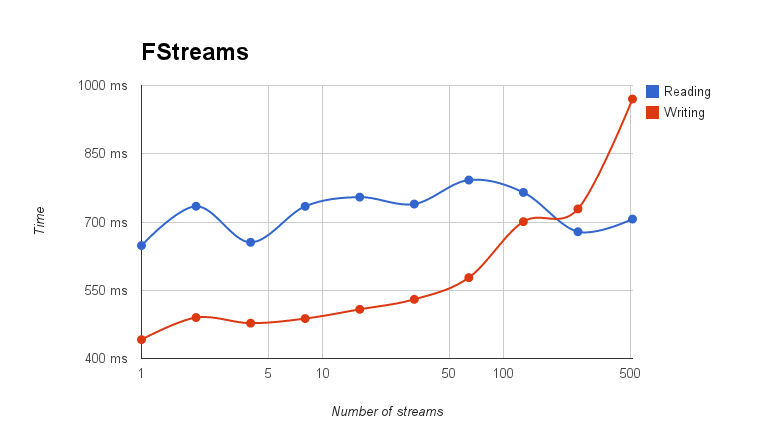
\includegraphics[width=90mm]{graphics/FS.png}

The implementation of these streams do not use a buffer - therefore the experiments only vary the number of streams.

The SingleItemStream is behaving as expected; the number of streams does not affect reading very much, and writing increases a bit per stream added, but nothing significant. 


The FStreams graph shows a wide variance in reading, but it stays within a 200ms range not dependant on the amount of streams. Writing on the other hand shows a rapid change in performance after exceeding 64 streams which seems surprising when the same did not happen for reading. 

\subsubsection{BufferedStreams and MMappedStreams}
For those streams, we first tried to find a good buffersize. Since the system have a pagesize of 4kb (1024 elements), we had a good idea that a buffer below that would be a waste of I/O. We varied the buffersize from 128 to 4M a got the following graph:

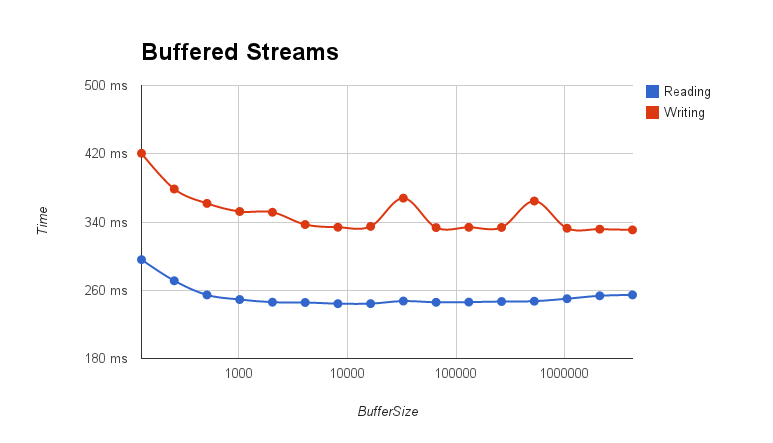
\includegraphics[width=90mm]{graphics/buffer_BS.png}
As expected, performance increases a lot until the page size of 1K. After that it stablizes and does not improve much - a buffer of size 1K seems sufficient.

For MemoryMappedStreams we where force to use a multiple of the page size (1024 elements), thus starting at 1K. Besides that, the experiment is similar to BufferedStreams and gives this graph:

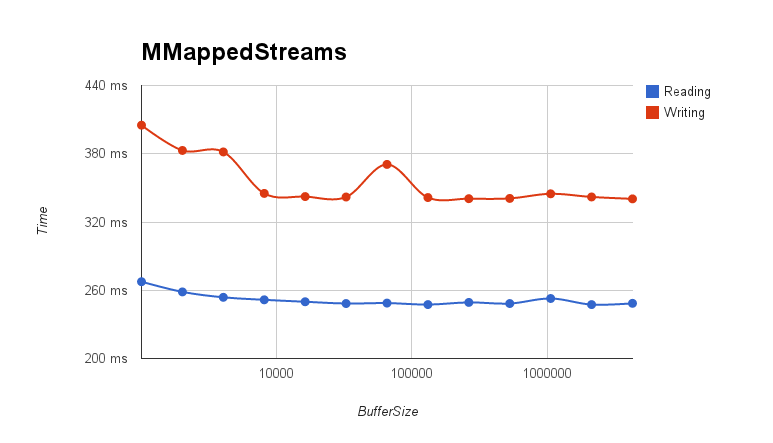
\includegraphics[width=90mm]{graphics/buffer_MMS.png}
Here it seems that a buffer of size 8K elements is a sweetspot.


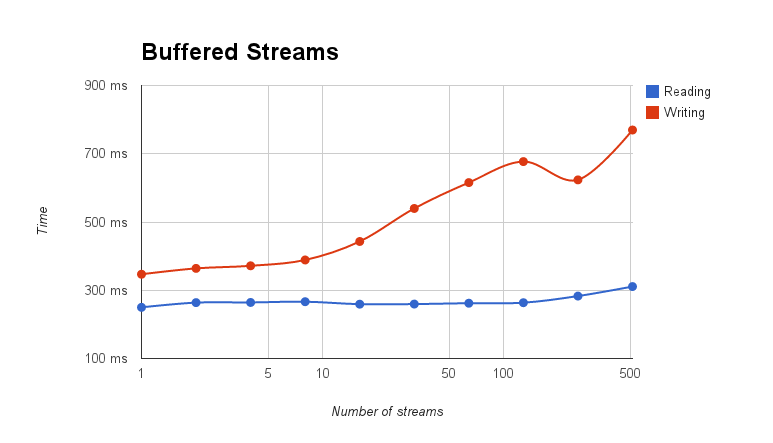
\includegraphics[width=90mm]{graphics/BS.png}
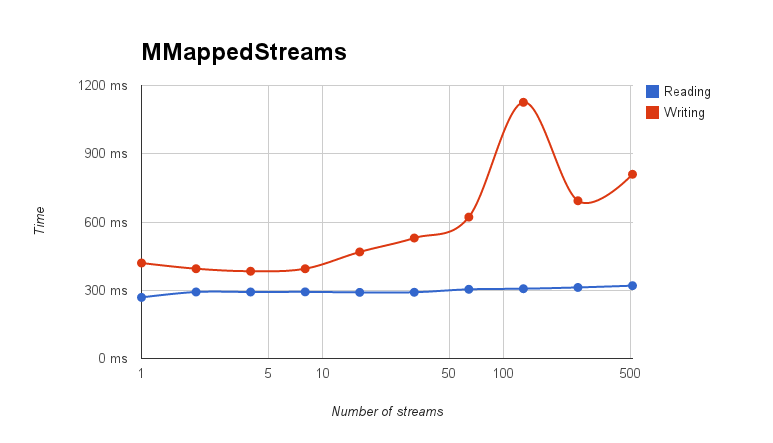
\includegraphics[width=90mm]{graphics/MMS.png}
These tests was done with a buffer size of 4K and 8K for the BufferedStreams and the MMappedStreams respectively.

The BufferedStreams implementation does reading reasonably well, with no significant increase in performance, the writing on the other hand does worse with more streams, with a slight drop around 256 streams, just to continue its performance decline. 

The MMappedStreams behaves similarly to the BufferedStreams, except that the running time is just slightly worse. The running time is practically unchanged for reading, while writing increases in running time the more streams we add. The interesting thing to note here though, is the large decline in performance with a buffer size of 128K, afterwards it drops again to expectable levels, and continues as such. Probably there have been some heavy I/O elsewhere which have had influence on the experiment. 

\subsubsection{Comparing the streams}
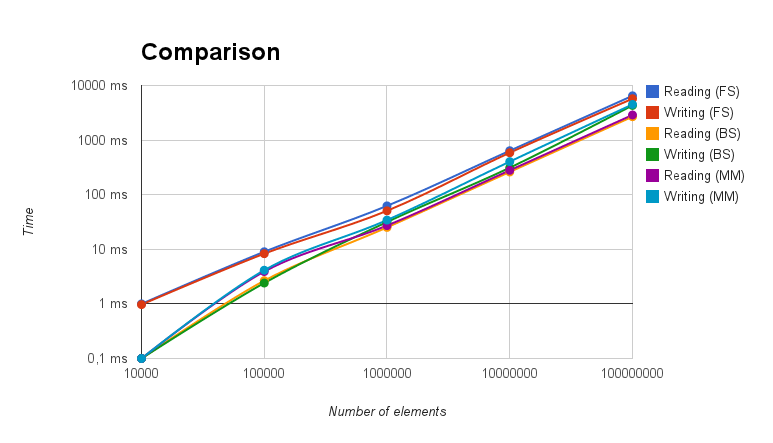
\includegraphics[width=90mm]{graphics/StreamCompare.png}
Our comparison graph for the stream implmentaions contain only three of the streams. The single item stream was so slow with large amounts of elements that we did not finish the tests for that implementation. The other streams are closer performance-wise as the graph shows. The streams based on \texttt{fread} and \texttt{fwrite} are clearly slowest which match up with what we expected. Our own buffered implementation slightly outperforms the \texttt{mmap} implementation which is why we ended up chosing that as the streams for our merge sort algorithm.

\subsection{ Finding merge sort parameters}
To find the best parameters ($b$, $m$ and $d$) for the merging algorithm, we first ran some simple tests to get at an idea of which boundries to look in. These were done with 1Mb of ram (i.e. 256K elements) In the setup we tried all combinations where:
\begin{align*}
	d &\in \{2, 8, 32\} \\
	m &\in \{16K, 64K, 256K, 1M, 4M\} \\
	b &\in \{1K, 4K, 16K\}
\end{align*}
These values where chosen a little arbitrary, but inspired by observations duing tests. The following values where obtained:
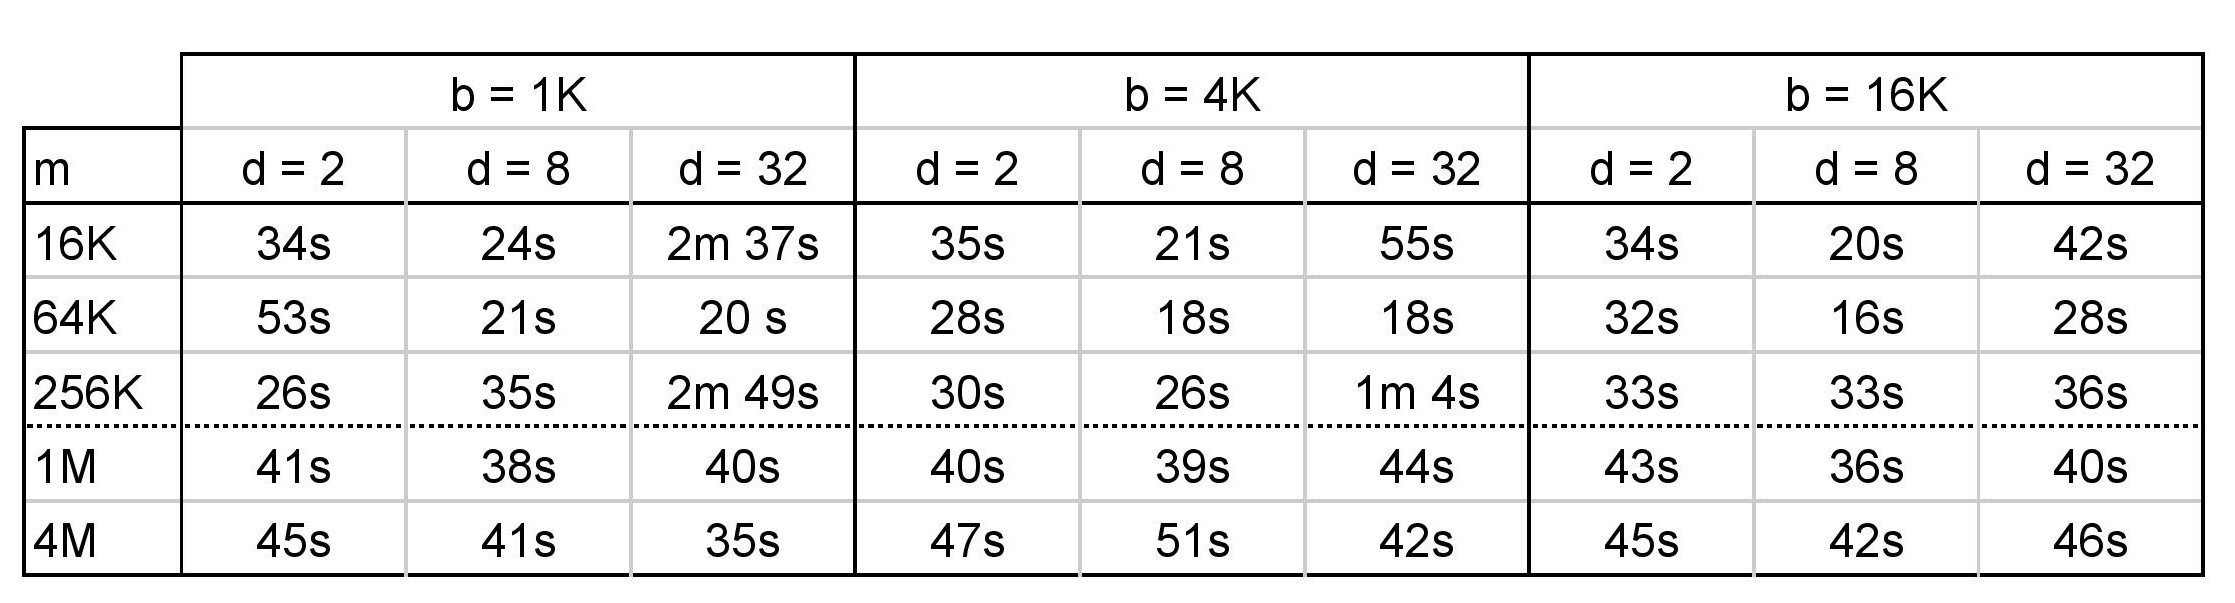
\includegraphics[width=90mm]{graphics/FindingParams.jpg}
The dotted line marks when m is growing bigger than the physical memory, and therefore swapping is needed. With the earlier experiment with the buffersize and the table above combined we concluded that a higher buffersize would not do much for our sorting algorithm. Furthermore it makes sense when we are dealing with a physical memory of size 256K.

We realized that the choices of $d$ and $m$ are independent. $m$ is only used for the splitting and $d$ for the merging. $m$ of course have effect on the number and size of streams created, but that does not affect the merging theoretically. Therefore we chose $m$ to a fixed size to find the best $d$ and vice versa. Test where executed five time for each value of $d$.

First we fix $m$ to 64K which gives the following graph:
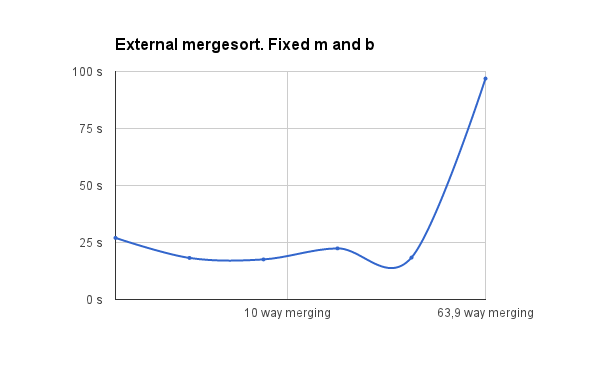
\includegraphics[width=90mm]{graphics/MergeSortFixedM.png}

From the graph we obtain an optimal $d = 32$. A quick test for values around $32$, indicates that $32$ is quite suitable.

Next we fix $d$ to 32 (lets use the best found) and that gives this graph:
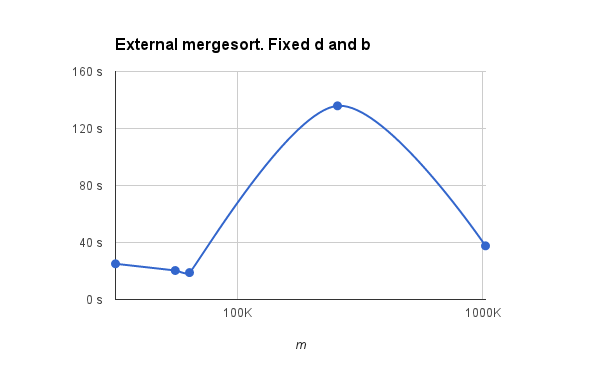
\includegraphics[width=90mm]{graphics/MergeSortFixedD.png}
Again we obtains an optimal value of 64K and again we perfom a quick test for values around 64K. It seems a little odd that 1024K only performs twice as slow as 64K, but it indicates that QuickSort (used to sort internally) performs okay when swapping and reduces the need of merges which uses quite an amount of I/O.

Now we obtained optimal (to some extent) parameters. These will be used for comparing the external mergesort with the internal quick- and heapsort.



